\chapter{How to Teach Your Machine}

Machine learning is an area of computer science in which we attempt to create intelligent systems that are able to make complex, human-level decisions. It has seen use in recent years in areas as diverse as self-driving cars, language processing, and automatic crop harvesting. In recent years, many machine learning techniques have started being applied to the realm of high-energy physics. Due to very high volumes of data production, especially for planned next-gen colliders such as the HL-LHC, and due the complexity involved in reconstructing each collision event, machine learning has increasingly been applied to tasks such as track reconstruction, vertex-finding, and jet identification, and played a part in the discovery of the Higgs. The field is extremely broad with many applications, so I will only attempt to describe a few basic ideas here.

\section{Basic Concepts}

Boiled down to its fundamentals, the goal of machine learning is to learn a function mapping. This function may map a single input (in what may be a high dimensional vector space) to a single output, as in an image classifier. It may also map multiple inputs to multiple outputs, as in the case of language translation, if we treat each word as an input or output. We may even have functions that produce a continuous stream of outputs for a continuous stream of inputs, as in a robotic system which produces actuator signals in response to its environment. Thus, the training step of machine learning may be seen as a process of function minimization, where we attempt to reduce the difference between our mapped outputs and our desired outputs.

For instance, a facial recognition system may take as its inputs a set of pixels originating from a camera or video feed, and output a pointer to a name in a database of people. A translation program may take a string of characters in one language as text input and output another string in a different language. A drone with obstacle avoidance may take input from visual systems and from mounted sensors, and output instructions to its various motors. Even an organic entity takes chemical, physical, and electrical inputs from its environment, and outputs signals to its muscles and organs, and can thus be modeled as a reinforcement learning agent.

We may classify some types of of machine learning algorithms by their training method. One type is supervised, where a system is fed a series of training examples, and is told explicitly what type of output the system should be attempting to obtain for each example. This is the case for an image classification algorithm, which may be fed many different input images, along with labels for each image. Another major class of machine learning algorithms is unsupervised learning. In this case, the algorithm is still fed input data, but is not told what the output should be. This is generally the case for clustering algorithms, such as those used for data compression and error/outlier detection. In addition, there are reinforcement learning algorithms, which process a stream of input and produce a stream of output, such as in the case of a video game playing AI. These algorithms are typically trained on a system of rewards which the algorithm gathers as it makes decisions in its environment.

Two common goals of machine learning algorithms are to perform classification and regression. In the case of classification, an algorithm is provided an input (or multiple inputs), and calculates a set of probabilities for which discrete classes the input may fall into. Image classification algorithms of course fall into this category. On the other hand, regression algorithms are used when there are not a discrete set of possible outputs. Rather, the net output is allowed to be unbounded (or at least continuous within a range), and the algorithm is graded based on how close its output gets to the target output. In some sense, language-based algorithms are typically classification-based, since there are a discrete number of words in a language to choose from. Image generation algorithms can be seen as regression-based, since we grade the generated image based on how close it is in vector space to a target output image.

\section{The Idea Behind Training}

As its name suggests, the field of machine learning is generally focused on how to get an algorithm to "learn" from input data, and as you've probably picked up from the preceding discussion, such learning is referred to as "training" the algorithm. A machine learning algorithm can take the form of a complicated expression with many tunable parameters. This expression may be in the form of a series of matrix operations, or as a chain of cut-based classifiers, or in general any other form of an input-output system with tunable components. In a supervised learning example, this algorithm begins with some initial (and probably randomized) parameters, and essentially spits out random outputs when given inputs. We train the algorithm by feeding it chunks of input data (called training data), and grading it based on comparing its outputs to the correct outputs. We tweak the parameters of the algorithm based on its performance after each training step. Once the algorithm is sufficiently trained, we can gauge the robustness of its performance on previously unseen data (referred to as test data).

The output grading step of the training process is quantified by calculating a "loss function", which is a function of the algorithm output and the correct expected output. In practice, for regression problems the loss function is often the L2 distance between the output and target output vectors. For classification problems the loss function is often cross entropy loss as shown in Equation~\ref{eq:cross_entropy}. In this equation, the sum is over all class indices $i$, $p$ is the target output distribution, and $q$ is the predicted output distribution. For example, if we are training an algorithm to recognize handwritten digits, we may have ten possible output classes (0-9). If we are then trying to recognize a handwritten digit 3, and our algorithm believes that the digit is a 2 with probability $15\%$ and a 3 with probability $85\%$, our cross entropy loss would be $-0\cdot\log(.15)-1\cdot\log(.85)$. As a concept, cross entropy measures how many bits would required on average to encode an event with a true probability distribution $p$ given an encoding scheme optimized for a probability distribution $q$. A high cross entropy indicates a large mismatch in underlying probability distributions.

\begin{equation}
\centering
H(p,q) = -\sum_{i} p_i \log q_i
\label{eq:cross_entropy}
\end{equation}

In all instances, our goal would be to tweak our algorithm such that the loss function is minimized over all training data. The specific way we do this depends on the algorithm, and we will discuss two common algorithms and their training methods in the next chapter.

\chapter{Basic Algorithms}

I will now talk about two very common machine learning algorithms, the boosted decision tree (BDT) and the neural net. Neural nets in particular form the basis of most modern machine learning, and all advanced architectures discussed in this thesis will be some form of neural network.

\section{BDTs}

Simply speaking, a decision tree is simply a series of branching paths based on input data, which one can follow to reach a conclusion. An example of a very simple decision tree is shown in Figure~\ref{decision_tree}. Decision trees are similar to how objects and signal regions are selected in a traditional high-energy-physics analysis. For example, one may ask whether an event has more than, less than, or equal to three leptons. If the event has exactly three leptons, one may ask whether the top two leptons have dilepton mass within a certain range, etc. Based on these decisions, an experimenter can decide what signal region an event belongs in. As another example, imagine that we are trying to determine what kind of particle we have seen in an event. We could ask whether the particle left a track in the inner detector, whether the amount of energy it deposited in the calorimeter is in a certain range, etc. Given a random ordered set of input variables, an optimal decision tree can be calculated for decisions made in that specific order.

A boosted decision tree is created by combining many different decision trees together \cite{BDT}. Any given decision tree can be very weak, containing only a small number of branches and a small maximum depth. However, by taking the weighted results of many decision trees together, we can get a more accurate result than can be achieved by any single tree. For the sake of space, the AdaBoost BDT training algorithm will not be discussed here.

\begin{figure}[t]
    \centering
    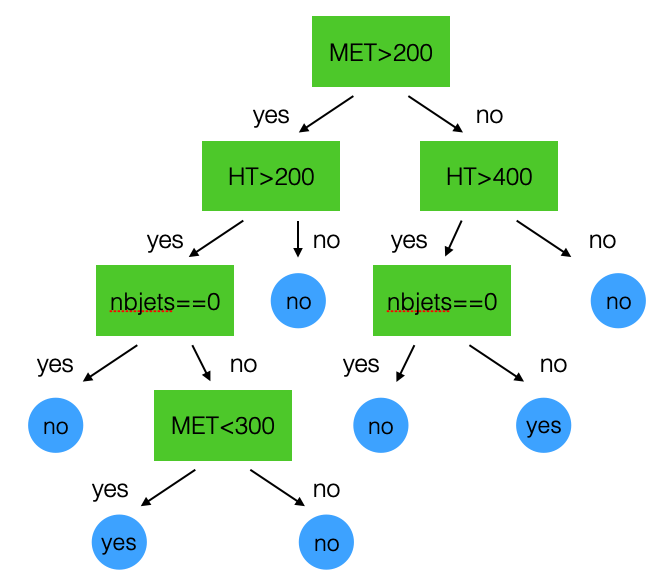
\includegraphics[width=0.5\linewidth]{images/decision_tree.png}
    \caption{An example of a decision tree that a child may use to classify a household pet.}
    \label{decision_tree}
\end{figure}

\section{Neural Nets}

A neural net is a machine learning architecture based on the physical structure of neurons in the human brain \cite{neural_net}. The basic unit of a neural net is a neuron, which has a numerical value, one or more inputs, and one or more outputs. These neurons are connected together so that the output of one neuron becomes the input of one or more other neurons. Here we will only consider simple feed-forward neural nets, where all the inputs to a neuron come from neurons closer to the beginning of the net, and all the outputs of that neuron go to neurons nearer the end of the net. That is, there are no "loops", and there are no connections between neurons at the same depth. The input values for an event form the first layer of neurons, and the output is derived from the last layer. Each link between neurons is associated with a "weight", or multiplicative constant. Each neuron is also associated with a "bias", or an additive constant. Letting $y_i$ be the value of the $i^{th}$ neuron, $w_{i,j}$ be the value of the weight between neurons $i$ and $j$, and $b_i$ be the bias associated with neuron $i$, we see that the value of a neuron is equal to $y_j = \sum{w_{i,j}y_i} + b_j$. Each neuron is also typically followed by a nonlinear "activation" function, so that the result of the entire net is not simply equivalent to a single matrix operation on the input. We see then that for a given set of weights and biases, we can calculate the output value for a net given any inputs.

In order to train a neural net, we use "back-propagation", meaning that for each event (or set of events) we perform gradient descent on each weight and bias in order to minimize the resulting loss function. Over the course of many events, the net can fall into a state where it produces the correct outputs with high accuracy. In this way, the neural net training is simply a form of function optimization. Many important topics, such as how to weight initialization, methods of gradient descent, net architectures, etc. will not be discussed in this paper.

\begin{figure}[t]
    \centering
    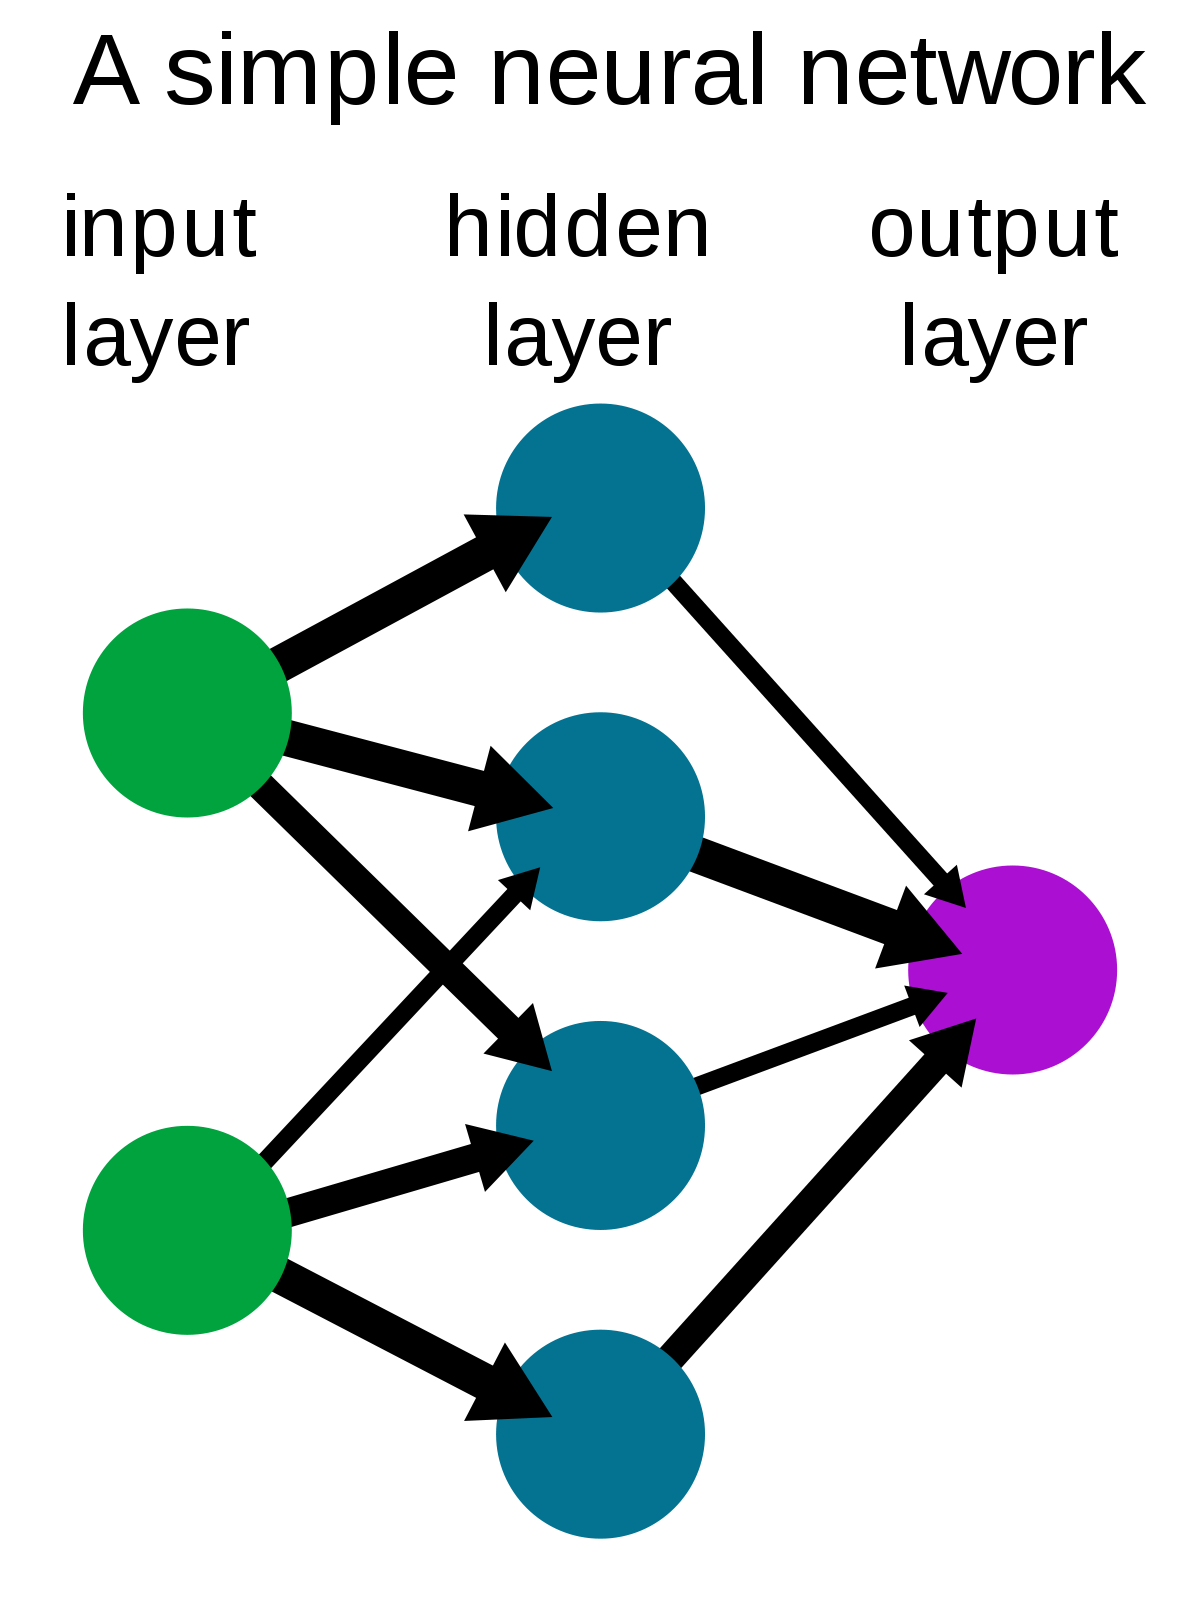
\includegraphics[width=0.5\linewidth]{images/neural_net.png}
    \caption{A diagram showing a typical densely-connected neural net.}
    \label{neural_net}
\end{figure}

\chapter{Advanced Architectures}

\section{Convolutional Nets}

\section{GoogLeNet}

\section{Generative Adversarial Nets}

\section{Recurrent Architectures}

\section{Deep Sets}

\section{Transformers}